Based on the definition of agility in the C2 context, the question "How to provide C2 agility?" is not completely explored and answered due to all complexity involved. The evidence found by NATO~\cite{FRANCE2014} in study cases and simulations is limited and they represent the state of the art and practice related to this subject. In particular, the C2 agility definition is inaccurate to explore the aspect of successfully and to address any notion of cost as a Quality Attribute (QA).

Indeed, to provide C2 Agility in dynamic scenarios in which members are performing a mission, it is necessary to guarantee efficient management of available resources to deal with context changes. The ability of the members to adapt themselves according to information received or obtained from the environment via sensors permits the system to keep running even under new circumstances. The challenge is adapting and maintaining quality attributes within acceptable levels.

Based on the state of the art on C2 Agility (cf. Chapter \ref{related}), considering the simulation context of \textit{in silico} and \textit{in virtuo} experiments\cite{simulation01}, we recall the two research problems mentioned in Chapter~\ref{introduction}:

\begin{itemize}
    \item (P1) Current works about C2 Approach Agility are limited;
    \item (P2) There is no evidence about C2 Maneuver Agility.
\end{itemize}

In particular, our focus is the software simulation based in \textit{in silico} experiments~\cite{simulation01}, where the environment, subject behavior and objects are computational models.





%%%%%%%%%%%%%%%%%%%%%%





In particular, one dimension of this gap is failing to address any notion of cost. In contrast, in real world C2  scenarios, cost is one of the most relevant aspects to be considered when assessing not only QAs but also mission feasibility. 

As these problems are wide and complex, we employ the Goal Question Metric (GQM) approach~\cite{gqm1} to guide the research questions identification and refinement. Figure~\ref{gqm} shows the three identified research questions. We omit the metrics, since these will be refined in the future and considered in the context of evaluation.  

Problem P1 motivates Research Question Q1. Indeed, Problem P1 summarizes the existing lack of QA measurement studies in scenarios where there is C2 Approach Agility, i.e.,  members adapt themselves but with no C2 Approach change. Current research addressed in Chapter~\ref{related} essentially deals only with mission or tasks accomplishment. Our base work, i.e., NATO Report~\cite{FRANCE2014}, considered as the state of the art in such analysis, did not consider any quality attribute, which simplified the employed simulation scenarios.

Problem P2 motivates Research Questions Q2 and Q3. In case of required change in the C2 Approach to deal with new circumstances, defined as C2 Maneuver Agility, current research does not present evidence on enabling this nor satisfying required QA levels. Indeed, simulations and observations conducted previously~\cite{FRANCE2014,Alberts2017,c2-02} only identify the need for C2 approach change, without describing any enabling mechanisms, and only address mission accomplishment. Cost considerations are ignored.

\begin{figure}[h]
\centering
\label{gqm}
\scalebox{.6}{


\tikzset{every picture/.style={line width=0.75pt}} %set default line width to 0.75pt        

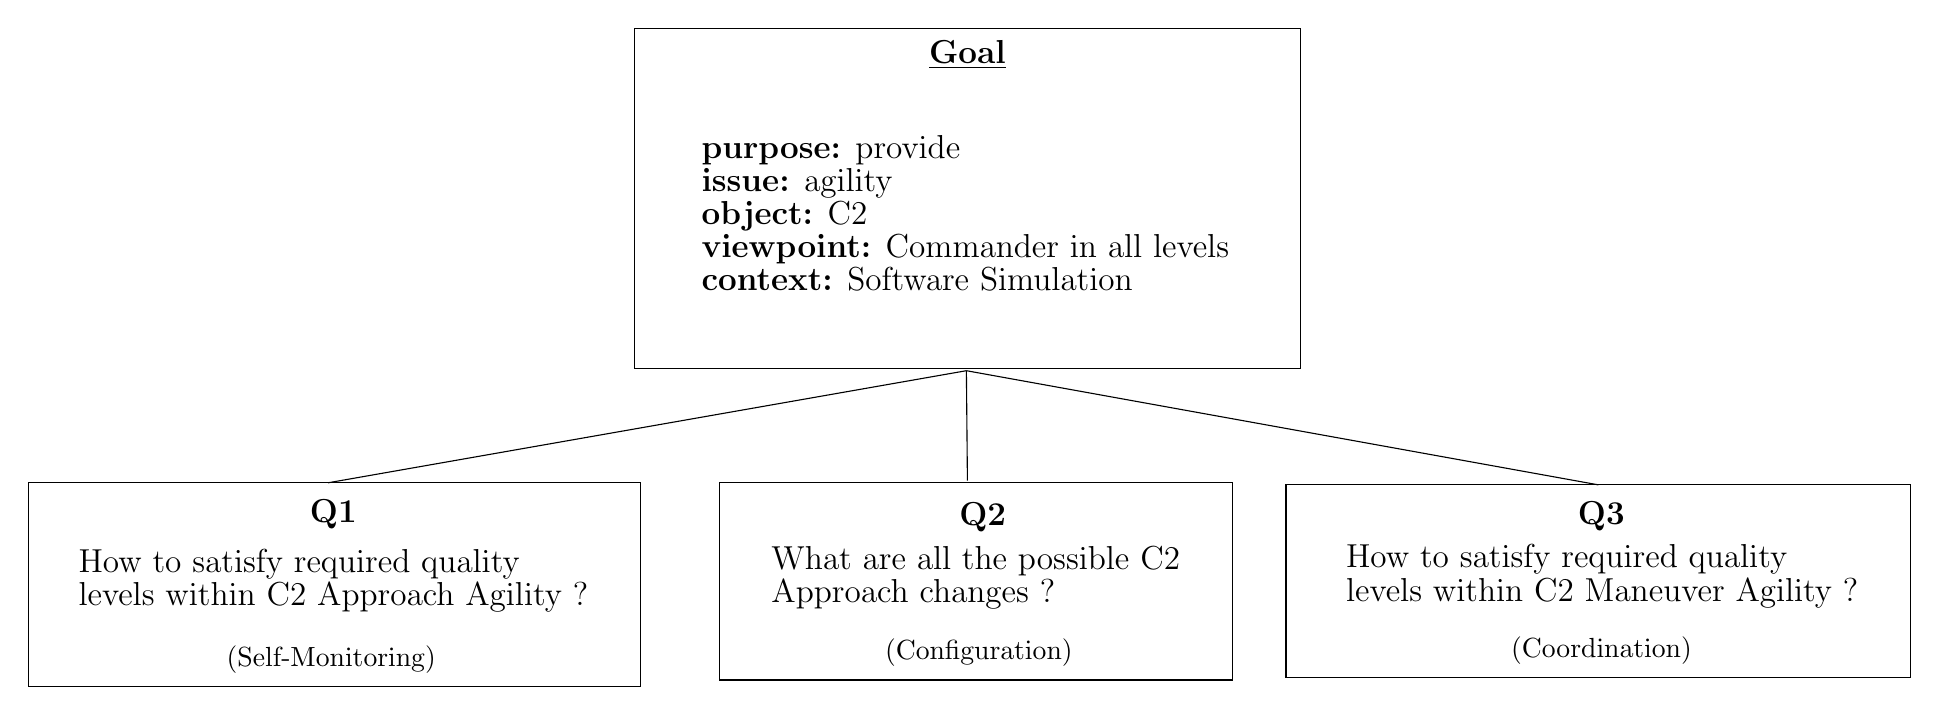
\begin{tikzpicture}[x=0.75pt,y=0.75pt,yscale=-1,xscale=1]
%uncomment if require: \path (0,334); %set diagram left start at 0, and has height of 334

%Flowchart: Process [id:dp9228173025001839] 
\draw   (295,2) -- (616,2) -- (616,166) -- (295,166) -- cycle ;
%Shape: Rectangle [id:dp9468174970136011] 
\draw   (609,222) -- (910,222) -- (910,315) -- (609,315) -- cycle ;
%Shape: Rectangle [id:dp09665993774558346] 
\draw   (3,221) -- (298,221) -- (298,319) -- (3,319) -- cycle ;
%Shape: Rectangle [id:dp4625317111731858] 
\draw   (336,220.67) -- (583,220.67) -- (583,316) -- (336,316) -- cycle ;
%Straight Lines [id:da1961523796551078] 
\draw    (455,167) -- (147.5,221) ;


%Straight Lines [id:da6120336423295578] 
\draw    (455,167) -- (759.5,222) ;


%Straight Lines [id:da223601999954537] 
\draw    (455,167) -- (455.5,220) ;



% Text Node
\draw (455.5,15) node  [font=\normalsize] [align=left] {\textbf{\underline{{\large Goal}}}};
% Text Node
\draw (150,236) node   [align=left] {\textbf{{\large Q1}}};
% Text Node
\draw (150,268) node   [align=left] {{\large How to satisfy required quality }\\{\large levels within C2 Approach Agility ?}};
% Text Node
\draw (459.5,266.67) node   [align=left] {{\large What are all the possible C2}\\{\large Approach changes ?}};
% Text Node
\draw (761.33,266) node   [align=left] {{\large How to satisfy required quality }\\{\large levels within C2 Maneuver Agility ?}};
% Text Node
\draw (760.92,237) node   [align=left] {\textbf{{\large Q3}}};
% Text Node
\draw (462.83,237.67) node   [align=left] {\textbf{{\large Q2}}};
% Text Node
\draw (454.5,91) node   [align=left] {{\large \textbf{purpose:} provide}\\{\large \textbf{issue:} agility}\\{\large \textbf{object:} C2}\\{\large \textbf{viewpoint:} Commander in all levels}\\{\large \textbf{context:} Software Simulation}};
% Text Node
\draw (461,303) node   [align=left] {(Configuration)};
% Text Node
\draw (149,306) node   [align=left] {(Self-Monitoring)};
% Text Node
\draw (761,302) node   [align=left] {(Coordination)};


\end{tikzpicture}}
\caption{GQM identifying Research Questions}
\end{figure}

Aiming at a more fundamental view on these research questions, we trace them to the agility enablers described in Chapter~\ref{background}, as indicated on Table~\ref{table:table06}. Correspondingly, flexibility, adaptability, and resilience are required to answer all the three questions, since they assure the system's ability to adapt according to new circumstances. Responsiveness provides required timely reaction and self-adaptation, whereas robustness promotes the system's ability of remaining in its initial configuration while maintaining  effectiveness even under perturbations or circumstance changes.

% Please add the following required packages to your document preamble:
% \usepackage[table,xcdraw]{xcolor}
% If you use beamer only pass "xcolor=table" option, i.e. \documentclass[xcolor=table]{beamer}
\begin{table}[ht]
\centering
\fontsize{10}{10}\selectfont
\caption{Tracing research questions into agility enablers}
\label{table:table06}
\begin{tabular}{|c|c|c|c|}
\hline
\rowcolor[HTML]{EFEFEF} 
\textbf{Agility Attributes} & \textbf{Q1} & \textbf{Q2} & \textbf{Q3} \\ \hline
Robustness & \bullet &  &  \\ \hline
Innovation &  &  &  \\ \hline
Adaptation & \bullet & \bullet & \bullet \\ \hline
Flexibility & \bullet & \bullet & \bullet \\ \hline
Resilience & \bullet & \bullet & \bullet \\ \hline
Responsiveness & \bullet &  & \bullet \\ \hline
\end{tabular}
\end{table}


%According to the aforementioned, there is the necessity of be able to analyze quality aspects in C2 context. Furthermore, it is not enough be agile in terms of fast execution, but it is necessary to keep results within requested levels and based on a constant monitoring and acting process. Analysis made by NATO considers only the mission completeness.